\section{Related work}

\subsection{Multilayer perceptron}
The multilayer perceptron is an artificial neural network (ANN) formed by
multiple layers, in such a way that it has the capacity to solve problems that
are not linearly separable, which is the main limitation of the perceptron (also
called simple perceptron).\\

\textbf{Linearly separable:} Linearly separable data is data that can be
separated by a line. To model this concept in a simple way, we are going to use
the logical functions AND and OR (which are linearly separable)
\cite{perceptron}.

\begin{figure}[H]
    \centering
    \begin{subfigure}[b]{0.8\textwidth}
        \centering
        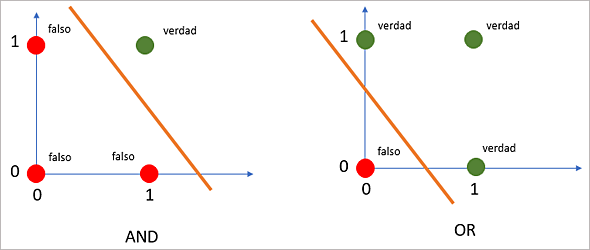
\includegraphics[width=\textwidth]{Figures/2. Related Work/perceptron.png}
        \caption{\textit{
                VANNIEUWENHUYZE, A. Artificial intelligence made easy: Machine
                Learning and Deep Learning at work. Recovered from:
                https://www.ediciones-eni.com/open/mediabook.aspx
            }}
    \end{subfigure}
\end{figure}

\subsection{Convolutional neural network}
Convolutional Neural Networks are a type of artificial neural networks where
"neurons" correspond to receptive fields in much the same way as neurons in the
primary visual cortex (V1) of a biological brain. This type of network is a
variation of a multilayer perceptron, however, because its application is
carried out in two-dimensional arrays, they are very effective for artificial
vision tasks, such as the classification and segmentation of images: which is
effective in detecting of objects and automation of protocols allowing automatic
driving in some models currently on the market.\\

Convolutional Neural Networks are a series of networks that were created
thinking about how the brain works, capable of learning at different levels of
abstraction: in the first layer, simple shapes, colors or edges are
differentiated; in the next layer of the document, combinations of borders and
colors can be distinguished; while the last layer looks at the shape in order to
figure out what exactly it is \cite{whatisacnn}. This is the process that follows when
classifying the images, but depending on the implementation there is a time
when the neural network is trained so that it learns to distinguish objects by
the properties in the image to be predicted. To do this, computers use filters
or lenses to see the different features: one sees the diagonal edges, another
the colors, etc. It works by passing filters over the entire image, scanning it,
and then defining and classifying it.

\subsection{General process}
Mainly it must be said that the detection of objects is not easy, generally the
human eye is capable of detecting objects, regardless of the type of light, if
it is blurred, the size of the object, the amount of the object it recognizes,
etc. Such a task is not easy for a machine to perform, usually you have to
turn a real world problem to a mathematical problem; Here convolutional networks
come into action, whose simplest interpretation is to treat the problem in
two-dimensional matrices and probabilistically. A convolutional network at the
time of being trained begins to detect similarities between image information
vectors through mathematical similarity techniques. The more iterations and
opportunities to obtain information from an image that describe the properties
in a mathematical way, the better trained the network will be to predict objects
in an image \cite{generalprocess}. for instance:

For everything the process has to do with detecting a car or a pedestrian on
the road, a vector would be used in this way, in the convolutional network to
correctly decide whether or not what it is holding is what it already knows.

\begin{figure}[H]
    \centering
    \begin{subfigure}[b]{0.6\textwidth}
        \centering
        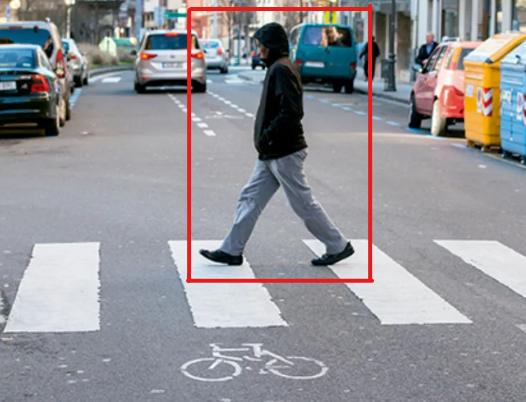
\includegraphics[width=\textwidth]{Figures/2. Related Work/person_detected.png}
        \caption{\textit{
                Person being detected
            }}
    \end{subfigure}
\end{figure}


\begin{equation}
    \left\{
    \begin{array}{ll}
        P_{c} \\
        B_{x} \\
        B_{y} \\
        B_{w} \\
        B_{h} \\
        C_{1} \\
        C_{2} \\
    \end{array}
    \right\}
    \left\{
    \begin{array}{ll}
        1  \\
        50 \\
        70 \\
        60 \\
        70 \\
        0  \\
        1  \\
    \end{array}
    \right\}
\end{equation}

\( P_{c} = \) If there is a car or a person.\\
\( B_{y} = \) Center of object perimeter \((y)\).\\
\( B_{x} = \) Center of object perimeter \((x)\).\\
\( B_{w} = \) perimeter width.\\
\( B_{h} = \) perimeter height.\\
\( C_{1} = \) If there is a car.\\
\( C_{2} = \) If there is a person.\\

But this vector would only represent a correct detection vector of a person in
an image with a region to predict. The previous problem is simplified because
there is still the part in which the image is analyzed to detect the possible
perimeters of objects to pass to the predictor and make its evaluation according
to its training.

In the previous exercise, it gives us an idea of what happens internally, the
convolutional network receives an image with vectors to be evaluated and gives
a prediction based on the analysis and what has been learned. Also the values of
the vectors are assigned according to the prediction and training of the
convolutional network. These vectors have to be organized in a specific way,
have a specific structure, and are analyzed differently depending on the
technique or approach we use to approach this problem.

So far we have seen some parts of the prediction process in images with
convolutional networks, recapitulating:

\begin{itemize}
    \item \textbf{Training of the convolutional network:} moment in which our
          network is going to be trained to classify specific objects, where it is
          going to define the parameters to decide if an object is one thing or
          another.
    \item \textbf{Boundary box detection:} moment in which our program will
          discard and detect the best positioned boundary boxes, which we will predict
          according to the training of the convolutional network.
    \item \textbf{Prediction of elements in the boundary boxes:} the boundary
          boxes found are analyzed and evaluated to find similarity between the
          elements known by the network.
\end{itemize}

\subsection{YOLO (You Only Look Once)}
You Only Look Once (YOLO) is a modern object detection algorithm developed and
published in 2015 by Redmon et al. \cite{yolo_1}. The name of the algorithm is
motivated by the fact that the algorithm only looks once at the image and
requires only one forward propagation pass through the neural network to make
predictions unlike other state of the art object detection algorithms which
work with region proposals and look at the image multiple times. YOLO uses a
single end-to-end convolutional neural network which processes RGB images of
size 448 x 448 and outputs the bounding box predictions for the given image:

\begin{figure}[H]
    \centering
    \begin{subfigure}[b]{0.8\textwidth}
        \centering
        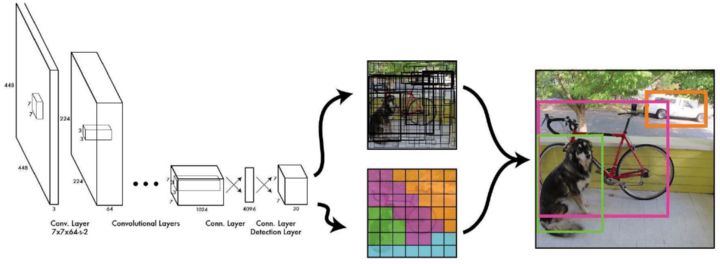
\includegraphics[width=\textwidth]{Figures/2. Related Work/yolo_1.png}
        \caption{\textit{Whole pipeline of YOLO's algorithm} \cite{yolo_images}}
    \end{subfigure}
\end{figure}

It basically reframes object detection as a single regression problem, straight
from image pixels to bounding box coordinates and class probabilities
\cite{yolo_2}. The algorithm divides the input image into an $S x S$ grid
(in the paper $S = 7$). For each grid cell it predicts B bounding boxes
(in the paper $B = 2$), where each bounding box consists of 4 coordinates and a
confidence score for the prediction, and C class probabilities per grid cell
taking the highest one as the final class. All of these predictions are encoded
as an $S x S x (B * 5 + C)$ tensor which is being outputted by the neural
network, as we can see in the following image.

\begin{figure}[H]
    \centering
    \begin{subfigure}[b]{0.6\textwidth}
        \centering
        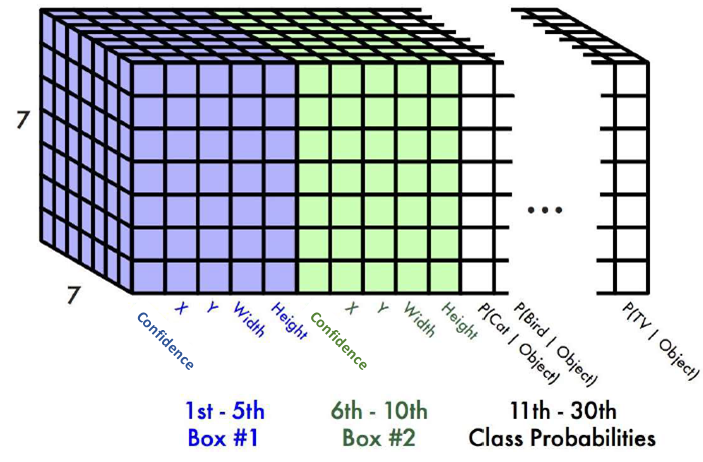
\includegraphics[width=\textwidth]{Figures/2. Related Work/yolo_2.png}
        \caption{\textit{The output tensor of YOLO} \cite{yolo_images}}
    \end{subfigure}
\end{figure}

What the algorithm finally does, is identifying objects in the image and mapping
them to the grid cell containing the center of the object. This grid cell will
be responsible for predicting the final bounding box of the object and will have
the highest confidence score.
In the example of the previous image, each cell of the $7 x 7$ grid is
represented by a vector of size 30 representing a particular area of the image.
Each vector contains 2 bounding box predictions (5 values each) and 20
conditional class probabilities $P(class|object)$. The first step upon extracting
a valid prediction is to choose the bounding box with the higher confidence
score and check if the confidence score is above a predefined threshold 
($threshold = 0.25$ in the paper) to output it as a valid prediction. This
confidence score represents the prior in the conditional probability for the
class prediction stating the probability that the given grid cell is the center
of an object with a correct bounding box. To extract the class prediction YOLO
outputs the conditional probability with the highest score. YOLO spatially
defines each bounding box by four coordinates ($X, Y, Width, Height$), where
$(X, Y)$ represent the center of the bounding box relative to the cell, while
$(Width, Height)$ represent the width and the height of the bounding box
relative to the whole image. Because of this, a bounding box can be bigger than
the cell where it was predicted. The cell is only used as the anchor point for
the prediction. One disadvantage of this approach is the fact that every cell
is able to predict only one object. If multiple objects are having their center
points in the same cell, only one will be predicted.

\begin{figure}[H]
    \centering
    \begin{subfigure}[b]{0.6\textwidth}
        \centering
        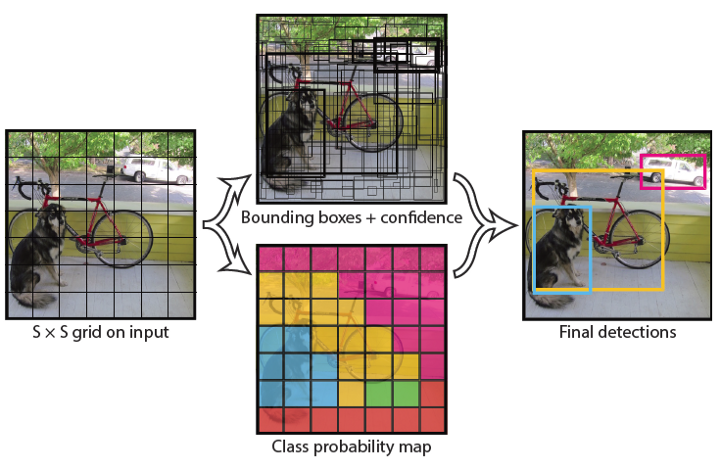
\includegraphics[width=\textwidth]{Figures/2. Related Work/yolo_3.png}
        \caption{\textit{$SxS$ grid and final detections} \cite{yolo_images}}
    \end{subfigure}
\end{figure}

\subsection{SSD (Single-Shot Detector)}

\subsection{R-CNN (Region-Based Convolutional Networks)}

\subsection{Fast R-CNN and Faster R-CNN}